\chapter{Hovedtekst}
I løbet af projektets to faser, inception og elaboration, har der været en løbende udvikling af projektets planlægning og produkt. Denne udvikling er sket på baggrund af ny viden, som gruppen har indhentet fra virksomhedsmøder, relateret undervisning og professionel vejledning. \\
En projektrammeplan er blevet brugt til at danne grundlaget for projektets planlægning. Den generelle projektrammeplan indeholdte fire afleveringer, samt grundlæggende milepæle, der skulle suppleres med gruppens egne mål. 
(Se interne bilag figur \ref{fig:tidsplanf}) \\
Første aflevering var gruppens projektforslag, som skulle bestå af de første ideer om problemstillingen i forhold til, hvordan den skulle formuleres, afgrænses og takles. (Se interne bilag \ref{in:projektforslag})\\
Anden aflevering var et Inceptionsdokument, som bestod af en grundlæggende analyse af projektet. Dette dokument skulle bl.a. indeholde systemets omfang, overordnede kravspecifikationer og prioritering af krav. (Se interne bilag \ref{in:inceptions})\\
Tredje aflevering bestod af det samlede arbejde fra første iteration af elaborationsfasen. Denne aflevering tog udgangspunkt i inceptionsdokumentet og startede med at opdatere projektets overordnede - og detaljerede kravsspecifikationer. Der blev udarbejdet statiske - og dynamiske analysediagrammer, samt statiske designdiagrammer. Ud fra disse planer, blev der udviklet et stykke software, som skulle være første skridt på vejen, mod projektets endelige kildekode.\\
Fjerde aflevering bestod af det samlede arbejde fra anden iteration af elaborationsfasen. Denne aflevering var en fortsættelse af første iteration, hvor der var fokus på at runde projektet af. Alle analyse- og designdiagrammer blev opdateret og der blev suppleret med et dynamisk designdiagram. Der var særligt fokus på at implementere den funktionalitet i kildekoden, som blev prioriteret højst, i forhold til fremtidig systemudvikling.\\
Det kommende afsnit vil gå i dybden med arbejdet og resultatet af det, som er blevet udført i første og anden iteration.

\section{Overordnet kravspecifikation}
Figur \ref{fig:overkrav} viser to forskellige systemafgrænsninger. 
Den ene systemafgrænsning er et login modul, som gruppen har valgt at simulere, da det originale Sensum har et login system tilknyttet. \\
Den anden systemafgrænsning, som er sagsforløb er det modul som gruppe har lagt fokus i. 
Her er der lagt størst fokus på opret sag og find sag, som er essentiel for systemet, da en sagsbehandler skal kunne oprette en sag på en given borger, inden den videre behandling kan forsætte. Dertil er det under sagsudredningen af borgerne også essentiel for en sagsbehandler at kunne gå ind i systemet og nemt finde en borger der er oprette en sag på.\\
Den brugsmønstermodel som blev udarbejdet i løbet af inceptionsfasen, har gruppen arbejdet ud fra, gennem elaborationsfasen. Den indeholder de brugsmønstre som gruppen har fundet nødvendige for at få netop modulet sagsudredning til at fungere.
\begin{figure}[hbt!]
  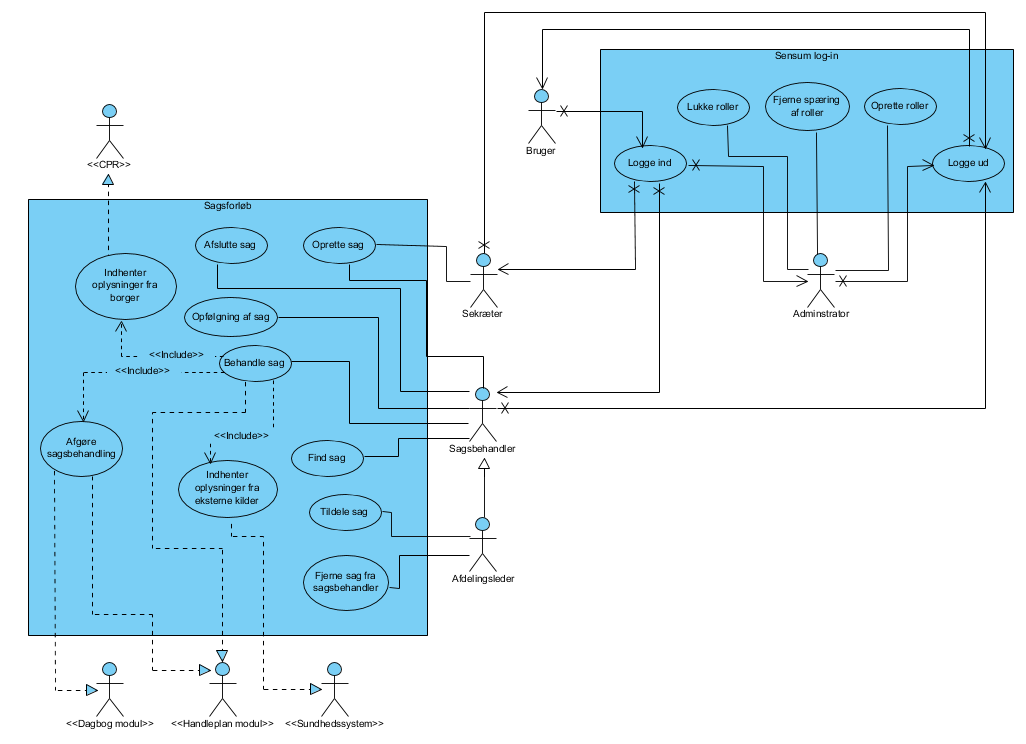
\includegraphics[scale = 0.4]{./PNG/krav/overkrav.PNG} 
  \caption{Overordnede brugsmønsterdiagram. For fuld størrelse se interne bilag afsnit \ref{sec:diverse} figure \ref{fig:fuldoverkrav}}
  \label{fig:overkrav}
\end{figure}

\section{Detaljeret kravspecifikation}
Ud fra den overordnede brugsmønsterdiagram (Se figur \ref{fig:overkrav}) er der blevet udvalgt forskellige brugsmønster, som er set som mere komplicerede brugsmønster end resten. Der vil blive lagt vægt på to krav i dette afsnit. Disse krav er opret sag og find sag. For at se alle af de detaljeret brugsmønstre se interne bilag figur \ref{tab:1} til figur \ref{tab:3} \\
\textbf{Opret sag} \\
Som vist på figur \ref{tab:opretSag} er der ikke noget specielt svært ved dette brugsmønster. I gennemgang af dette kom der mange forskellige ting op, omkring hvad der ville være fornuftigt at skulle bruge til at oprette sagen. Det endte ud med at der skulle bruges en person, som sagen omhandle samt en grund til at sagen skulle eksistere.
\begin{figure}[hbt!]
\begin{longtable}{|p{18cm}|}
\hline
\textbf{Brugsmønster: }Opret sag \\
\hline
\textbf{ID: }1 \\
\hline
\textbf{Primære aktører: }Sagsbehandler, afdelingsleder, administrativt personale\\
\hline
\textbf{Sekundære aktører: }CPR\\
\hline
\textbf{Kort beskrivelse: }En aktør kan oprette en sag, som gemmes i systemet. \\
\hline
\textbf{Prækonditioner: }Aktør skal være logget ind.\\
\hline
\textbf{Hovedhændelsesforløb: }\newline 
Starter når en borger henvender sig til kommunen. \\
1. Aktør indtaster CPR nummer, borgers navn, begrundelse for henvendelse. \\
2. Gemmer indtastet data.	
\\
\hline
\textbf{Postkonditioner: }sag oprettet\\
\hline
\textbf{Alternative hændelsesforløb: }\\
\hline
\end{longtable}
\caption{Brugsmønster for opret sag}
\label{tab:opretSag}
\end{figure}\\
\textbf{Find sag}\\
Brugsmønsteret find sag (Se figur \ref{tab:findSag}) er til for at finde en vilkårlig sag. Dette skal kunne ske ud fra sagsnummer fra sagen, navnet på personen sagen omhandler og deres CPR-nummer. Det er vigtigt at brugsmønsteret kan åbne en specifik sag, eller stoppes hvis ikke det er den rigtige søgning. 
Alle krav kan findes i interne bilag afsnit \ref{sec:diverse} figur \ref{fig:krav} og figur \ref{fig:ikkeKrav} 
\begin{figure} [hbt!]
\begin{longtable}{|p{18cm}|}
\hline
\textbf{Brugsmønster: }Find sag \\
\hline
\textbf{ID: }3\\
\hline
\textbf{Primære aktører: }Sagsbehandler\\
\hline
\textbf{Sekundære aktører: }none\\
\hline
\textbf{Kort beskrivelse: }Skal kunne søge i sager og få en sag vist\\
\hline
\textbf{Prækonditioner: }Der skal være oprettet en eller flere sager\\
\hline
\textbf{Hovedhændelsesforløb: }\\
Starter når den primære aktør skal finde en sag.\\
1. Skal søge en sag på sagsnummer, CPR nummer, eller navn.\\
2. Vise en liste over de sager som blev fundet.\\
3. Valgt sag kan åbnes.\\
\hline
\textbf{Postkonditioner: }\\
\hline
\textbf{Alternative hændelsesforløb: }\\
\hline
\end{longtable}
\caption{Brugsmønster for find sag}
\label{tab:findSag}
\end{figure}
\section{Første iteration}

Formålet med elaborationsfasen er at skabe en prototype af produktet MMMI(Se ordliste). Denne udvikling sker på baggrund af inceptionsfasen (Se interne bilag afsnit \ref{in:inceptions}), hvor der blev opstillet en række krav til projektet.  For at kunne nå de mål bliver der lavet nogle mindre iterationer herunder analyse, design, kode og test som udarbejdes, basseret på den overordnede kravspecifikation. 

\section{Analyse}
Der er blevet lavet en række diagrammer over de forskellige detaljeret brugsmønster.\\
Der er to forskellige typer af analyse diagrammer, der er de dynamiske og de statisk.
\subsection{Statiske side af analysen}
\begin{figure}
  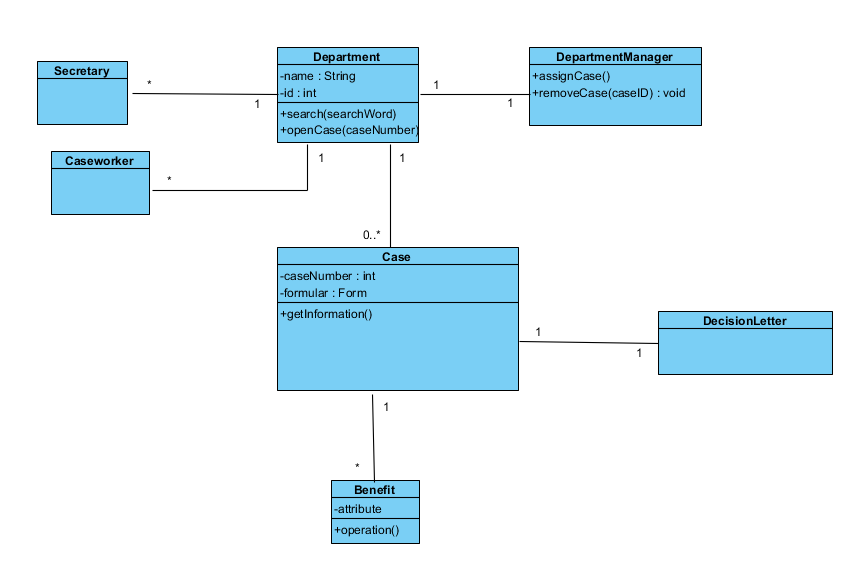
\includegraphics[width=\linewidth]{./PNG/analyseKlasseDiagram.PNG} 
  \caption{Analyse klasse diagram.}
  \label{fig:AKlasse}
\end{figure}



\subsection{Design}
\subsubsection{DesignStatisk}
\begin{figure}[h]
\includegraphics[width = \linewidth]{./PNG/design/designKlasseDiagram.PNG}
\caption{Klasse diagrammfuld størrelse se interne bilag afsnit \ref{sec:diverse} figur \ref{fig:fuldDesignKlasseDiagram}}
\label{fig:desginklasse}
\end{figure}
Diagrammet \ref{fig:desginklasse} beskriver de klasser vi har fundet, der skal implementeres i systemet. Hver klasse har attributter og en del skal have skrevet getter / setter-metoder til, men for at diagrammet ikke skal blive for stort og uoverskueligt, blev der valgt at undlade dem.\\
Diagrammet er blevet designet med tanker på en tydelig lagdeling og repræsentere systemets domænelag. Der blev besluttet at ”Department”-klassen skulle benyttes som facadeklasse til præsentationslaget, mens datahandler interfacet bruges til kommunikation mellem domæne- og persistentslag.
Department – Facade klasse\\
Der var særligt fokus på attributterne: ”id” af typen int og ”caseMap” af typen Map<String, Case>. Det var tænkt at ID skulle bruges til at godkende adgangen til sager i databasen, for at imødekomme projektets ”Dataafgrænsning”. ID er af typen int, for at holde den simpel. Kravet til dataafgrænsningen er, at en arbejder der henter information omhandlende en borger, ikke må blive gjort opmærksom om sager, der administreres af andre afdelinger end arbejderens egen.\\
Tanken bag attributten ”caseMap”, var at department skulle have en liste af case-objekter som kunne bruges til at hente de relevante informationer frem for at sende dem til præsentationslaget. Der blev valgt at bruge et Map da Key/Value-strukturen gør det nemmere at finde en sag. Den Key der blev valgt til caseMap er caseNumber og skal bruges til metoden openCase(…)\\
Klassens metoder, som ”search(…)”, ”openCase(…)”, mm. er designet til at håndtere den logik, som controllerne fra præsentationslaget skal bruge. Metoderne repræsentere de funktioner som er ønsket i det grafiske userinterface (GUI).\\
Når metoden ”search(…)” kaldes, skal logikken først hente data fra persistenslaget. Dette sker gennem Interfacet PersistanceInterface som opretter et objekt af klassen ”SearchCase”, som er designet til at være en placeholder i domænelaget, for data der er relevant til en brugers søgeord.\\
\textbf{SearchCase – Placeholder klasse}\\
Klassen består af en constructor med attributterne: ”citizen”, ”caseNumber”, ”caseStatus”, ”date”, ”reason”, ”employeeName” og ”employeeID”. Disse informationer er ikke et udtryk for alt der ligger i en sag, men er nok til at præsentere en borgers sag og derefter hente de resterende informationer. \\
Hvis der er et ønske om at hente den fulde sag, gøres dette ud fra ”caseNumber”-attributten gennem ”openCase(…)” metoden, fra ”Department”-klassen . Den data der er relateret til en sag, hentes fra persistenslaget, gennem interfacet ”PersistanceInterfase”.\\
\textbf{PersistanceInterfase – Datahandler interface}\\
For at behandle dataflowet mellem persistenslaget og domænelaget, er der blevet designet et interface med metoderne: ”create()”, ”read()”, ”update()” og ”delete()”. Disse metoder blev valgt for at kunne lave, hente, ændre og slette data, som opbevares i persistenslaget. For at domænelaget kan sende dataforespørgsler til persistenslaget, skal der implementeres anonyme klasser af det påkrævede interface, som så kalder den ønskede interfacemetode.\\ 
\textbf{Case : Employee : Citizen – Objektklasser}\\
Objektklasserne blev designet med tanken om at præsentationslaget og persistenslaget, skulle arbejde med konkrete instanser af disse. Persistenslaget skulle tilføje den data, som var forbundet med objektet, som blev kaldt gennem domænelaget. Præsentationslaget skulle registrere indholdet i objekterne, pakke det ud og præsentere det som ønsket. \\
\textbf{JobTitle – Rollebaseret kontrol}\\
Superklassen ”JobTitle” blev designet til at kontrollere en given medarbejders rettigheder i systemet. Der blev taget udgangspunkt i tre jobstillinger, som blev skrevet op som subklasser - sekretær, sagsbehandler og afdelingsleder. Når en medarbejderklasse blev oprettet, skulle det være et krav, at de fik tildelt en stilling (JobTitle). Denne stilling skulle kunne ændre sig i systemet, f.eks. på grund af en forfremmelse, uden at medarbejderen skulle registreres på ny i systemet.\\
Stillingen som en medarbejder tildeles, skulle begrænse systemets funktionalitet, så de kun havde adgang til de områder, som var nødvendig til at udfører deres opgave. En sekretær skulle f.eks. ikke kunne andet end at registrere en person, som søger behandling samt årsagen for at der søges. En sagsbehandler skulle have fuld adgang til relevante sager, dvs. kun sager der er oprettet i den afdeling sagsbehandler er tilknyttet. En afdelingsleder skulle kunne det samme som en sagsbehandler, men også kunne styre hvilke sager de forskellige sagsbehandlere skulle arbejde på.\\
\textbf{Multiplicitet/Multiplicity – Klassernes forbindelser}\\
Forbindelserne mellem klasserne i designdiagrammet, består primært af aggregeringer. Klassen ”Employee” er forbundet med en many-to-one aggregering til klassen ”JobTitle”. Dette er blevet valgt, da objekter af klassen ”JobTitle” ikke skal blive slettet, hvis et ”Employee”-objekt fjernes. Tanken der ligger til grund for dette, er at ”JobTitle” kan være forbundet til flere forskellige ”Employee”-objekter. \\
Klassen ”Department” er forbundet til ”Employee” med to aggregeringer. Første aggregering er ”employeeList”, som er en one-to-many relation. Aggregeringen er blevet lavet, for at indikere at der kan være mange der arbejder i samme afdeling, men det skal stadig være muligt at slette en ”Department”, uden at slette ”Employee”-instanserne. Anden aggregering er ”departmentManager”, som er en one-to-one relation. Denne aggregering er blevet lavet, for at demonstrere at der altid skal være en leder i en afdeling. Igen skal det være muligt at slette en ”Department”, uden at det sletter ”Employee”.\\
Klassen ”Department” er forbundet til ”Case” med en enkelt aggregering. Dette er en one-to-zero-or-more forbindelse, som betyder at en afdeling ikke altid har nogen sager, men en sag er altid forbundet til en afdeling. Aggregeringen blev valgt, da en sag ikke forsvinder, hvis afdelingen bliver fjernet. \\
Klassen ”Case” er forbundet med to aggregeringer til klassen ”Citizen”, som også er forbundet med en komposition tilbage igen. Den første aggregering der er lavet, er en zero-or-many-to-zero-or-many relation, som omhandler en sags henvisning. En person kan blive henvist af nul eller flere personer, omhandlende det samme problem og på samme måde er det også muligt for en person at have henvendt sig for at få oprettet nul eller flere sager. Anden aggregering er lavet af samme grund som kompositionen er. En ”Citizen” kan have en til flere sager i gang på en gang, men en sag skal altid være angående en enkelt ”Citizen”. Aggregeringen er anvendt da det skal være muligt at fjerne en ”Case” fra systemet, uden at fjerne den ”Citizen” sagen omhandler. Kompositionen er derimod blevet brugt, da en ”Case” altid vedrører en ”Citizen”, og hvis denne fjernes fra systemet, skal de relaterede ”Case”-objekter fjernes, da de ikke længere vedrører nogen.\\
Klassen ”SearchCase” er forbundet med en komposition fra interfacet ”PersistanceInterfase”. Da et interface ikke kan instantieres, har det ikke nogen multiplicitet. Kompositionen er blevet valgt, da ”SearchCase” ikke fungere uden interfacet, og forsvinder derfor, hvis interfacet fjernes.\\


\subsection{DesignDynamisk}


\subsection{Implementering}
Målet med første iteration var at skabe et domain lag der havde de funktionalitetter som var nødvendige for systemet så det kunne fungere. Dette blev gjort så gruppen havde en bedre forståelse for hvordan systemet skulle se ud. I det følgende tekst er der lagt vægt på brugsmønsterende opret sag og find sag. Igennem første iteration var der lavet to klasse (case og department) der implementeret begge brugsmønster. ”case” håndteret hvad for noget data der skulle gemmes i en sag, mens ”department” holdt styr på hvad for nogle sager der var og hvordan man skulle finde dem.  Nedenfor ses de forskellige attributter der var I ”case” klassen(ref), udover dem var der gætter og sætter på attributterne. 
\\INSERT KODE\\
Der bruges et map til at holde den data der ændre og skrives ind, mens der er en status på om sagen er lavet, I gang eller færdig. Der er og kan kun være en person, sagen omhandler så der er simple variable, mens der kan være flere der fortæller det kan være en god ide at den her person for noget hjælp. Det gjorde at der skulle være en list over disse personer. \\
For at kunne se hvad der skrives ud I præsentationslaget går det igennem facaden som er afdeling. Det er også her at alle de forskellige sager vil være gemt I denne iteration. Der bliver genererer et sagsnummer hvor det også er tydeligt at se for os hvilken afdeling sagen tilhørere. \\ 
For at oprette en sag skal der bruges en person og oprette sagen på hvilket gør at funktionen skal enten få en person ind eller få information nok ind så den kan selv oprette den person sagen omhandler. Neden for er ses det hvordan dette er blevet håndteret(ref). 
\\INSERT KODE\\
Som det kan ses I koden nedenfor(ref) ses det hvordan klassen ”department” finder en sag den skal bruge en ”string” som kunne være CPR-nummer for personen den omhandlede, sagsnummeret for sagen og navnet på personen sagen omhandler. 
\\INSERT KODE\\
Som det kan ses I koden er der ikke blevet returneret en sag, men en list af sager. Dette er blevet gjort af flere årsager. Et par af de årsager er at en person kan have flere sager og mere end en person hedder det samme. Det kan også være en bruger af systemet ikke kender hele navnet så det skulle være muligt at få alle med fornavnet Anders tilbage, dette nåede ikke at blive implementeret I denne iteration. 



\subsection{Test}
\begin{figure}[hbt!]
\begin{lstlisting}
public static void main(String[] args) {
	while (!quit) {
                rollInfor();
                text = sc.nextLine().toLowerCase();

                switch (text) {
                    case "secretary":
                        Employee trine = detDepartment.createEmployee("trine", 
                        252525, "secretary");
                        commands(trine);
                        break;
                    case "caseworker":
                        Employee mads = detDepartment.createEmployee("mads", 
                        353535, "caseworker");
                        commands(mads);
                        break;
                    case "departmentmanager":
                        Employee martin = detDepartment.createEmployee("martin", 
                        262626, "departmentmanager");
                        commands(martin);
                        break;
                    case "quit":
                        System.out.println("Du quiter");
                        quit = true;
                        break;
                    default:
                        System.out.println(text + "Er ikke en kommando\n");
                        break;
                }
\end{lstlisting}
\caption{tekst under figuren}
\label{kode:1main}
\end{figure}
Der blev ikke lavet unit test på første iteration, da det ikke blev set som en nødvendighed. Det der blev fokuseret på var systemtest som skulle sikre at forståelsen med projektet og hvordan de forskellige brugsmønstre ville fungere i et færdigt system. Der blev fundet flere fejl/mangler igennem systemet. Vist på koden (Se figur \ref{kode:1main}) kan det ses at der bliver lavet en ny ”employee” hvilket skyldes det ikke var lavet så den kunne huske mere end en ad gangen. Det kan ses I figur \ref{kode:1commando} er det de forskellige kommandoer som kan bruges returneres det vil derefter testes om personen der er logget ind. \\
Dette blev den eneste rigtige test da dette kom ud på at få ideen til hvordan systemet skulle fungere helt på plads så databasen og præsentations laget kunne blive lagt på. 
\begin{figure}[hbt!]
\begin{lstlisting}
public static String loop() {
        while (true) {
            Scanner s = new Scanner(System.in);
            String t = s.nextLine().toLowerCase();

            switch (t) {
                case "back":
                    return t;
                case "create case":
                    return t;
                case "close case":
                    return t;
                case "add information":
                    return t;
                case "assign case":
                    return t;
                case "reassign case":
                    return t;
                default:
                    System.out.println(t + " Er ikke en kommando \n");
            }

        }
    }
\end{lstlisting}
\caption{loopet der ser om kommandoen kan er rigtig}
\label{kode:1commando}
\end{figure}
Dette blev den eneste rigtige test da dette kom ud på at få ideen til hvordan systemet skulle fungere helt på plads så databasen og præsentations laget kunne blive lagt på.
\newpage


\section{Anden iteration}

\subsection{Hvad skal der gøres}
Efter at domain laget var lavet skulle der laves en brugergrænseflade samt et data lag. 


\subsection{Analyse}

\subsubsection{Statisk analyse}
\begin{figure}[htb!]
  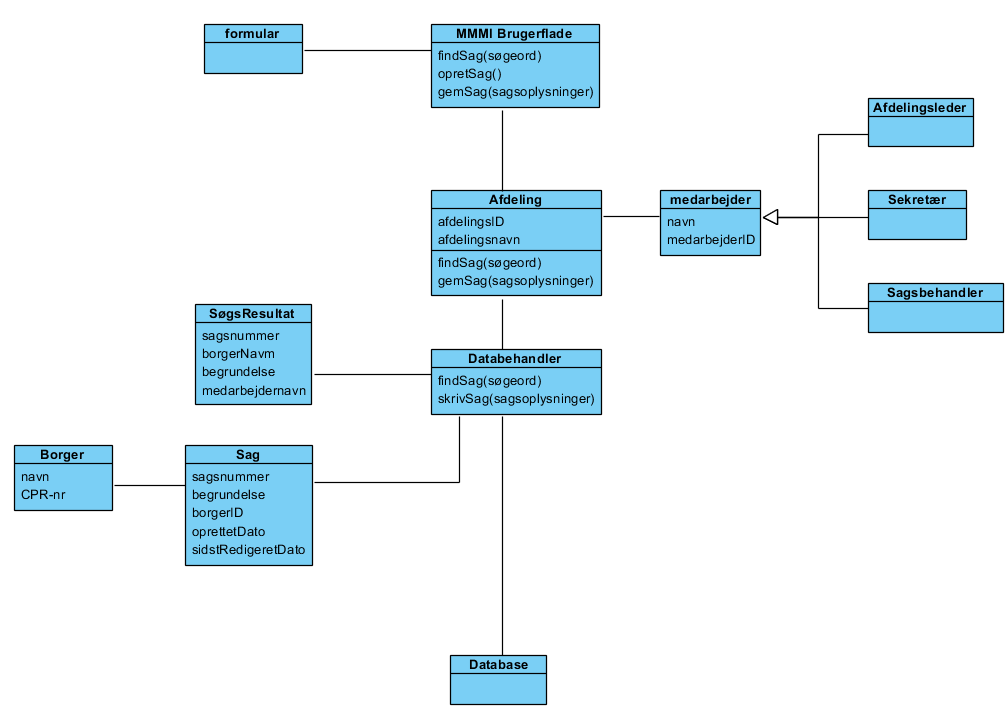
\includegraphics[scale = 0.7]{./PNG/analyse/analyseklassediagramOpdateret.PNG} 
  \caption{Analyse klasse diagram opdateret til anden iteration}
  \label{fig:2analyseklasse}
\end{figure}
Da der har været fokus på at få integreret en database og en funktionel grafisk brugergrænseflade i 2. iteration, består de primære ændringer i den statiske analyse, af arbejdet med at revidere klassediagrammet, med henblik på at tilføje persistens og præsentation. Der er bl.a. blevet ændret på hvordan de tre klasser der repræsenterer ansatte, og klassen der repræsenterer borgere, beskrives. \\
Der blev valgt at gå væk fra en overordnet abstrakt klasse (Se figur \ref{fig:AKlasse})kaldet ”Person”, som ”Borger”, ”Afdelingsleder”, ”Sekretær” og ”Sagsbehandler” klasserne arvede fra. En abstrakt klasse kaldet ”medarbejder” blev lavet, som ”Afdelingsleder”, ”Sekretær” og ”Sagsbehandler” arvede fra i stedet, og holdt ”Borger” som en separat klasse. Dette betød at ”Borger” fik navn og CPR-nr. som attributter, til forskel fra 1. iteration hvor den kun havde CPR-nr. og arvede navn fra ”Person”. Yderligere blev medarbejderID flyttet til superklassen, da alle arvende klasser skulle bruge den. \\
Det blev droppet at beholde ”Afgørelsesbrev” som klasse, da det gav mere mening at lægge den i præsentationslagets klasse ”Formular”, som også repræsenterer alle andre formularer der beskrives i VUM.\\
Klassen ”Sag” er blevet rykket ned til datalaget og kan tilgås gennem Databehandler klassen, som er den klasse der repræsenterer datalaget og skal varetage al kommunikation med databasen.\\
De vigtigste metoder og attributter, på diverse klasser, er blevet opdateret i forhold til den nye viden, der er blevet indsamlet gennem 2. iteration. Der er blevet lavet nye metoder er på klassen (Se figur \ref{fig:2analyseklasse})”MMMI Brugerflade”, som er ”findSag”, ”opretSag” og ”gemSag”. På klassen ”Afdeling” er metoderne ”findSag” og ”gemSag” blevet lavet og på klassen ”Databehandler” er ”findSag” og ”skrivSag” blevet lavet. De nye attributter som er tilføjet, er ”begrundelse”, ”borgerID”, ”oprettetDato” og ”sidstRedigeretDato” på ”Sag”. \\
Den nye klasse ”SøgsResultat”, bruges til at holde data samlet i forbindelse med en given søgning af en sag. De attributter som vises i klassen ”SøgsResultat”, repræsenterer en begrænset delmængde af hvad der gemmes når en sag oprettes, men det er nok til at en bruger vil være i stand til at identificere en given sag for at åbne den.\\
Klassen Database repræsenterer den postgresql database er blevet implementeret i iteration 2.

\subsubsection{Dynamisk analyse}
I anden iteration er der blevet udarbejdet operationssekvensdiagrammer i forhold til ”opretSag()”, ”opdaterSag()” og ”find()”. \\
Operationen ”opretSag()” (Se afsnit \underline{\ref{opret} opretSag}) og ”opdaterSag()” (Se afsnit \underline{\ref{opdaterSag} opdaterSag}) er operationer der stammer fra opretSag fra første iteration. I de pågældende sektioner vil der beskrives de overvejelser der blevet fortaget i forhold til de to operationer samt beskrivelse og vurdering. \\
Operationen find() er den operation der stammer fra ”findSag()” fra første iteration. I afsnit \underline{\ref{find} find} beskrives der overvejelserne om f.eks. fra ”findSag()” til find() og beskrivelse samt vurdering af operationen.\\ 
\textbf{opretSag():} \label{opret} \\ 
Operationen ”opretSag()” er den funktion der opretter en sag i systemet. Der gjort overvejelser om at håndtere opdaterSag() i samme funktion som ”opretSag()”, men det ville ikke give mening samtidig med at det ville gøre diagrammet uoverskueligt. Derfor er de adskilt i to operationer. \\
\begin{figure}[htb!]
  \includegraphics[scale = 0.5]{./PNG/analyse/opretsag2.PNG} 
  \caption{Sekvensdiagram for opret sag opdateret til anden iteration Se interne bilag \ref{sec:diverse} figur \ref{fig:2fopretsag}}
  \label{fig:2opret}
\end{figure}
I figur \ref{fig:2opret}. begynder funktionen ved at en sagsbehandler eller sekretær vælger ”opretSag()”. Brugergrænsefladen returner en sagsåbningsformular, som skal udfyldes. Når sagsbehandleren har indtastet sagsoplysningerne vælger sagsbehandler at gemme sagen. Operationen ”gemSag()” sender besked til Afdeling som derefter benytter operationen ”skrivSag()” til Databehandleren og til sidst sender Databehandleren beskeden videre til databasen. Databasen returner en bekræftelse tilbage til Databehandleren som returner den igennem Afdeling og til sidst fortæller aktøren at sagen blev oprettet. \\
Ved at anvende ”opretSag()” operationen har en sagsbehandler eller sekretær mulighed for at vælge en formular og udefra den gemme den og dermed oprette en ny sag. Oprettelsen sker når borgeren henvender sig og dermed kan sekretæren eller sagsbehandleren oprette en sag på den pågældende borger. For at kunne håndtere om en borger allerede har en sag eller om der findes oplysninger om borgen, benyttes ”find()” operation, som kan læses i afsnit \underline{\ref{find} find}\\
\textbf{opdaterSag():} \label{opdaterSag}\\
Operationen ”opdaterSag()” med en kombination af ”find()” operationen gør det muligt for en aktør at kunne finde en specifik sag og dermed åbne den og opdatere den. \\
\begin{figure}[htb!]
  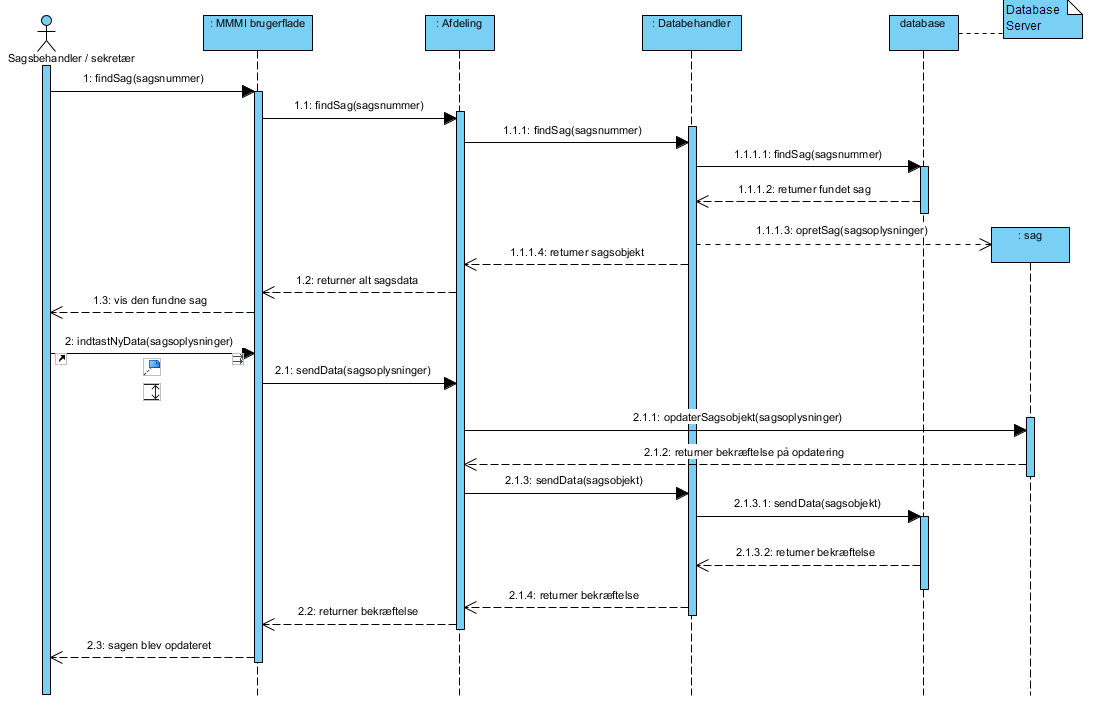
\includegraphics[scale = 0.62]{./PNG/analyse/opdaterSag.PNG} 
  \caption{Sekvensdiagram for opdater sag opdateret til anden iteration}
  \label{fig:2opdater}
\end{figure}
I figur \ref{fig:2opdater} ses det at en sagsbehandler eller sekretæren vælger at fremsøge en sag. ”findSag()” beskeden bliver sendt igennem afdelingen og databehandleren. Databehandleren sørger for at sende beskeden til databasen og fremskaffe den søgte sag. Denne returneres til databehandleren og der bliver oprettet et sagsobjekt. Dette sagsobjekt returneres til afdelingen og herefter til brugerfladen og til sidst bliver den vist til brugeren. Når brugeren vælger at ”indtastNyData()” til det pågældende sagsobjekt, med de pågældende sagsoplysninger sendes til afdelingen via operationen ”sendData()”. Afdelingen sørger for at opdater sagsobjektet igennem beskeden ”opdaterSagsobjekt()” hvor sag returner sagsobjekt med sagsoplysningerne og det sagsobjekt og data sendes til Databehandleren igennem beskeden ”sendData()” som derefter sender besked til databasen om at gemme de nye oplysninger. Databasen returner en bekræftelse igennem databehandleren, afdelingen og til sidst sendes det til brugerfladen som så bekræfter overfor aktøren at sagen blev opdateret. \\
Det vurderes at denne operation er en væsentlig del af sagsforløbet og skulle kunne muliggøre for en sagsbehandler eller sekretær at kunne opdatere en sag ved at kombinere operationen med at finde en sag først og derefter opdatere den. \\
\textbf{find():} \label{find}\\
\begin{figure}[htb!]
  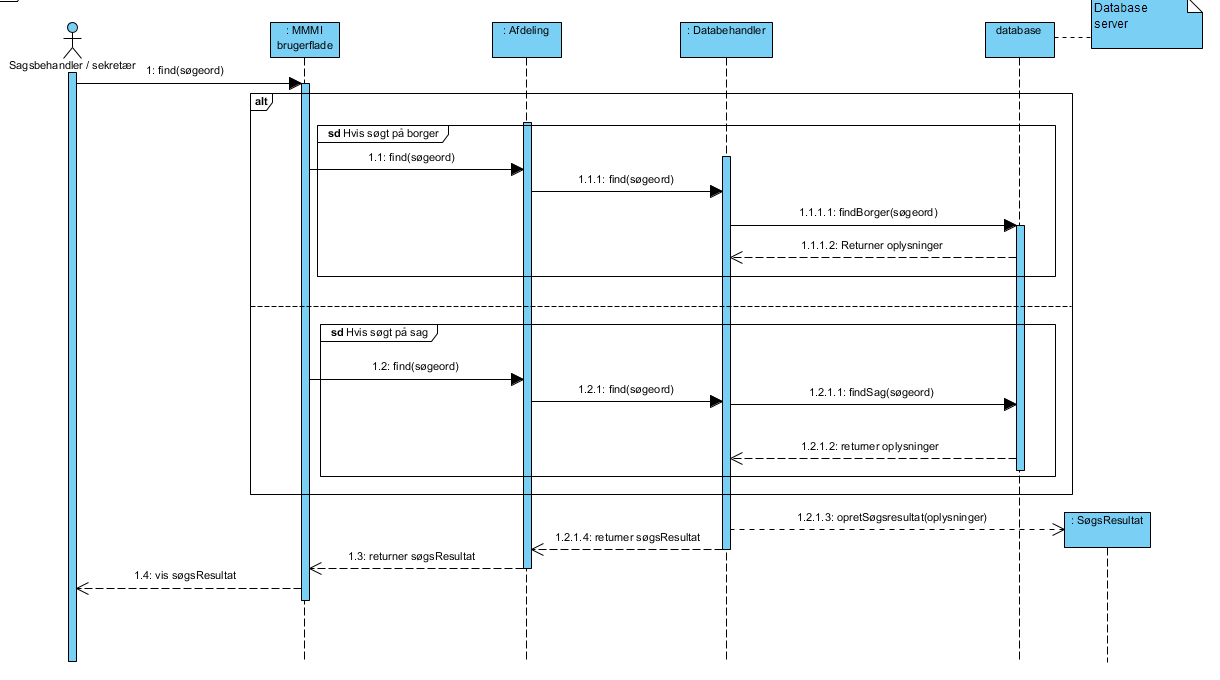
\includegraphics[scale = 0.56]{./PNG/analyse/find.PNG} 
  \caption{Sekvensdiagram for find sag opdateret til anden iteration}
  \label{fig:2find}
\end{figure}
Tanken med ”findSag()” i første iteration afsnit … har været at kunne fremsøge en pågældende sag frem. Der har været overvejelser om at kunne fremsøge en borger og en sag, fra en enkelt operation. Derfor blev ”findSag()” operationen lavet om til en mere general operation kaldt ”find()”.\\
I figur \ref{fig:2find} vælger en sagsbehandler eller sekretær at finde en sag eller borger baseret på et søgeord. Operationen ”find()” sender besked til grænsefladen. Baseret på den pågældende søgning, hvis det er en borger eller en sag der søges på, sendes ”find()” besked videre fra Afdelingen til Databehandleren der sørger for at sende besked til databasen, hvor der efterfølgende sendes svar fra databasen til Databehandleren der så baseret om det er en sag eller borger der er søgt på, opretter et SøgsResultat objekt, som Databehandleren sender tilbage. Afdelingen sørger for at sende beskeden til brugerfladen som til sidst viser søges resultatet til aktøren. \\
At kunne finde en sag frem eller en specifik borger er en vigtig funktion og dermed en vigtig operation for en sagsbehandler eller sekretær. Denne operation hjælper med at kunne finde sag på en pågældende borger og dermed hjælpe mere effektivt, ved at kunne hente alle sagsoplysninger. \\ 


\subsection{Design}
\subsubsection{Den statisk side af dasign}
Designdiagrammet i projektets anden iteration, blev opdateret med flere klasser og en tydelig lagdeling. En klar adskillelse af præsentations-, domæne- og persistenslaget er blevet illustreret og indeholder også subsystemernes klasser, med attributter og metoder. Det er valgt at getter og setter metoder ikke vises i diagrammet, da det ville gøre det meget større og sværere at overskue. (Se interne bilag figur \ref{fig:opklasse})\\
For at få et samlet overblik se interne bilag \ref{sec:diverse} figur \ref{fig:opklassemedlog} og figur \ref{fig:opklasse}\\ \\
\textbf{Præsentationslaget}
\begin{figure}[htb!]
  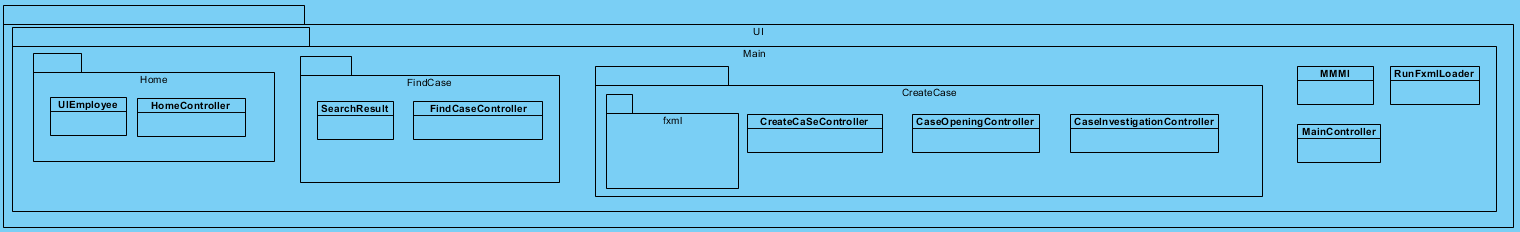
\includegraphics[width = \linewidth]{./PNG/design/UIopdateretKlassediagram.PNG} 
  \caption{Der blev valgt at undlade beskrivelsen af kontrollernes indhold og FXML-dokumenterne i subsystemet UI (Præsentationslaget), for at gøre diagrammet mere overskueligt. Præsentationslaget er blevet illustreret med pakker, som indeholder kontrollere og FXML-dokumenter for specifikke funktioner, samt klasserne som styrer systemets GUI.}
  \label{fig:2pre}
\end{figure}
\\\textbf{MainController – Præsentations controlleren}\\
Klassen ”MainController”, er systemets primære FXML-handler. Den blev lavet så det var muligt at skifte funktionalitet, på baggrund af et brugerinput, i samme root-node.\\\\
\textbf{RunFxmlLoader – Præsentationsmetoden}\\
Klassen ”RunFxmlLoader”, indeholder funktionaliteten som bruges til at skifte FXML-dokumenter. Den bliver arvet af ”MainController”, og implementere, som det eneste, metoden der bruges til at skifte ”pane”, i systemet.\\\\
\textbf{MMMI – Main Class}\\
Programmet køres gennem MMMI klassen, da det er programmets main class.\\\\
\textbf{CreateCase – Dokumentstyring og præsentation}\\
Subsystemet ”CreateCase”, blev designet til at begynde oprettelsen af nye sager i systemet og styre præsentationen af sagsdokumenter, samt brugerinteraktionen med disse. I slutningen af anden iteration var ”CreateCase”, pakket med kontrollerne ”CreateCaseController”, ”CaseOpeningController” og ”CaseInvestigationController”, samt FXML-pakken ”fxml”, som var pakket med de tilsvarende FXML-dokumenter.\\ 
Controlleren ”CreateCaseController”, blev designet til at styre bevægelsen mellem sagsdokumenter, samt at gemme brugerindtastet information fra disse dokumenter. Navngivningen kunne virke misvisende, i forhold til at controlleren bruges til at skifte mellem dokumenter, men peger på funktionaliteten bag gem funktionen. Når en given bruger benytter gem funktionen i en sag, sender controlleren de brugerindtastede informationer til domænelaget, for at få det registreret i systemdatabasen. \\
Hvis en sag gemmes for første gang i systemet, vil informationen som sendes gennem systemlagene, oprette en ny sag i databasen, som derefter modtager informationen. Controlleren er blevet navngivet efter denne proces, men har i sig selv kun at gøre med brugerinput og kommunikationen med domænelaget.\\
Controlleren ”CaseOpeningController”, er designet til at pakke informationerne indtastet i FXML- dokumentet ”caseOpeningNew”, og derefter sende det videre til ”CreateCaseController”, når en given bruger benytter gem funktionen.\\
Controlleren ”CaseInvestigationController”, har at gøre med informationen fra FXML-dokumentet ”caseInvestigation”. Controlleren er designet ligesom ”CaseOpeningController”, da de begge er designet til at håndtere information fra FXML-dokumenter, som er designet efter dokumenterne fra VUM. (Anon., 2019) \\
Designet af ”CreateCase”, var planlagt med fremtidig udvikling i tankerne, for at lave og implementere de dokumenter fra VUM, som mangler.\\ \\
\textbf{FindCase – Sagsrelateret søgning} \\
Subsystemet ”FindCase”, er designet til at håndtere et brugerinput, i form af en søgning, og præsentere information relateret til søgeordet. Subsystemet består af klassen ”SearchResult” og controlleren ”FindCaseController”, samt FXML-dokumentet ”findCase”.\\
Klassen ”SearchResult”, er en placeholder som fyldes med den data, der hentes på baggrund af en given brugers søgeord. Controlleren ”FindCaseController”, henter informationen som ”SearchResult”, består af og præsentere dem gennem FXML-dokumentet ”findCase”.\\\\
\textbf{Home – Systemets startside} \\
Subsystemet ”Home”, er designet til at håndtere systemets startside. Subsystemet består af klassen ”UIEmployee”, som er en placeholder klasse for medarbejderen der er logget ind i systemet og controlleren ”HomeController”, samt FXML-dokumentet ”home”.\\
Klassen ”UIEmployee”, er en placeholder klasse, som fyldes med information relateret til medarbejderen der er logget ind i systemet. Controllerklassen ”HomeController”, bruger informationen fra ”UIEmployee”, til at finde de relevante informationer som vedrør medarbejderen og præsentere dem gennem ”home”-dokumentet.\\\\
\textbf{Domænelaget}
\begin{figure}[htb!]
  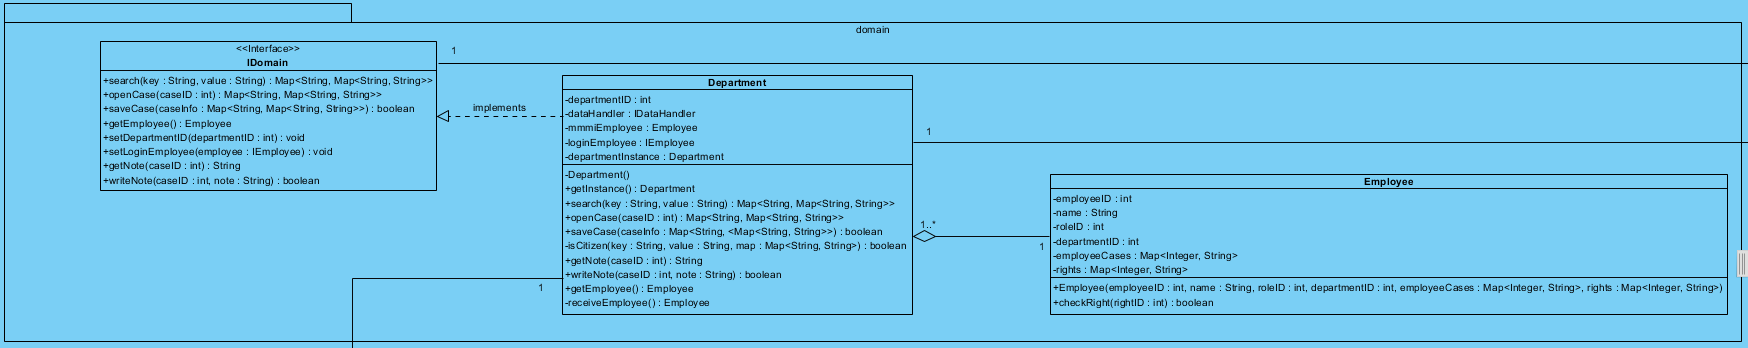
\includegraphics[width = \linewidth]{./PNG/design/domaeneOpdateretKlassediagram.PNG} 
  \caption{Domænelaget er blevet designet med to klasser, med attributter og metoder, og et interface.}
  \label{fig:2dom}
\end{figure}
\\\textbf{IDomain – Provided interface}\\
IDomain interfacet bruges til at vise præsentationslaget hvilke metoder der er tilgængelige i domænelaget, hvad de returnerer samt hvilke attributter der er nødvendige for at benytte metoderne. Interfacets metoder bliver implementeret i ”Department” klassen.\\\\
\textbf{Department – Facadeklasse}\\
Klassen ”Department” har en private constructor “Department()”, attributterne ”departmentID”, ”dataHandler”, ”mmmiEmployee”, ”loginEmployee” og ”departmentInstance”, samt metoderne ”getInstance()”, ”search(…)”, ”openCase(…)”, ”saveCase(…)”, ”isCitizen(…)”, ”getNote(…)”, ”writeNote(…)”, “getEmployee()” og “receiveEmployee()”.\\
For at imødekomme projektets underspørgsmål ”Hvordan sikres det at aktøren kun har adgang til det aktøren har brug for?” og dataafgrænsningen fra sagsudredning i semestercasen, er der blevet lagt stor vægt på attributten “departmentID”. \\
Dette ID tildeles via en setter metode, ”setDepartmentID(…)”, når en medarbejder logger ind i systemet. Singleton designpattern blev valgt, da der er nødvendigt at være sikre på at det er det samme ”Department”-objekt der arbejdes med gennem hele systemet.\\\\
\textbf{Employee – Dataklasse, repræsenterer den medarbejder der er logget ind}\\
Klassen ”Employee” er designet til at håndtere tjek af rettigheder i forhold til forskellige medarbejderroller. Når en bruger logger ind i systemet, sendes der en employeeID til ”Department” som kalder persistenslaget for at få data om medarbejderen for at oprette en instans af Employee.\\
Dette gøres for at det kan være muligt at der er styr på hvem der er logget ind, samt have mulighed for at tjekke rettighederne som medarbejderen har gennem metoden ”checkRight(…)”.\\ \\
\textbf{Persistenslaget}
\begin{figure}[htb!]
  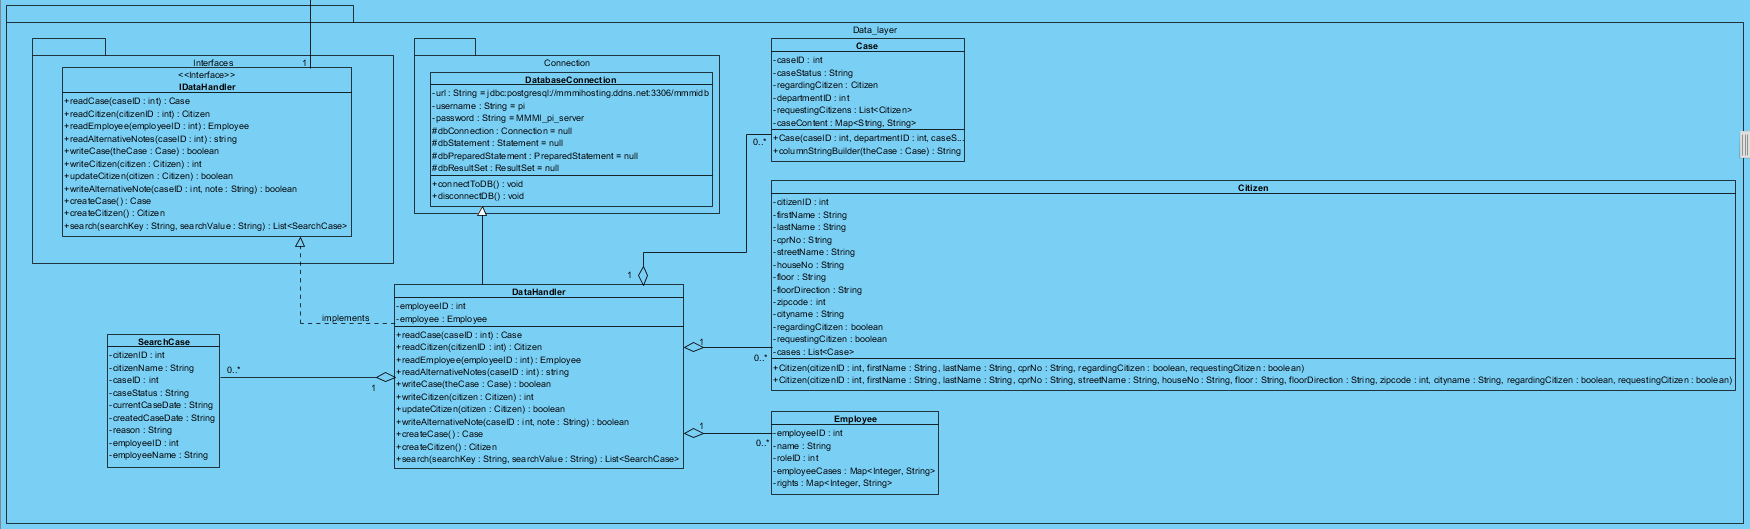
\includegraphics[width = \linewidth]{./PNG/design/datalagKlassediagram.PNG} 
  \caption{Persistenslaget er blevet designet med seks klasser og et interface.}
  \label{fig:2dataklassediagram}
\end{figure}
\\ 
\textbf{IDataHandler – Provided interface} \\
Interfacet ”IDataHandler”, bruges til at tillade og etablere kontakten mellem domænelaget og persistenslaget. Metoderne som interfacet består af implementeres i ”DataHandler” klassen og kaldes i domænelaget, når databasen skal kontaktes.\\
\textbf{DataHandler – Facadeklasse}\\
Klassen ”DataHandler”, er blevet designet til at håndtere dataforespørgsler sendt fra domænelaget og behandle dem som ønsket i systemets database. Klassen implementerer ”IDataHandler” interfacet og metoderne der følger med, som specificeres så data bliver hentet og/eller gemt, når de bliver kaldt fra domænet.\\
Når der skal hentes data fra databasen, er metoderne ”readCase(…)”, ”readCitizen(...)”, ”readEmployee(…)”, ”readAlternativeNotes(…)” og ”search(…)”, blevet designet for at kunne tilgå specifikke koloner, så den relevante information kan blive hentet. \\
Designet er lavet så at, når der skal gemmes data i databasen, benyttes metoderne ”writeCase(…)”, ”writeCitizen(…)”, ”updateCitizen(…)” og ”writeAlternaticeNote(…)”. Metodekaldet der skal bruges, afhænger af hvilken information der ønskes gemt. \\
Klassens associationer består primært af aggregeringer, med multipliciteten one-to-zero-or-many. ”DataHandler” er forbundet med aggregeringer til klasserne ”SearchCase”, ”Case”, ”Citizen” og ”Employee”. \\\\
\textbf{SearchCase – Placeholder til data fra “search(…)”}\\
Klassen ”SearchCase” indeholder udelukkende attributterne ”citizenID”, ”citizenName”, ”caseID”, ”caseStatus”, ”currentCaseDate”, ”createdDateCase”, “reason”, “employeeID”, “employeeName”.  Klassen bruges når der søges i databasen med metoden ”search(…)”, til at indeholde de data der er relevant at vise brugeren, i forhold til at kunne vælge den rigtige sag at åbne.\\\\
\textbf{Employee – Dataklasse, repræsenterer en medarbejder og alle dennes tilknyttede sager i afdeling}\\
Klassen ”Employee” indeholder udelukkende attributterne ”employeeID”, ”name”, ”roleID”,\\ ”employeeCases” og ”rights”. \\\\
\textbf{Case – Dataklasse, repræsenterer en sag}\\
Klassen ”Case” indeholder attributterne “caseID”, “caseStatus”, “regardingCitizen”, “departmentID” som alle skal bruges for at oprette en ny sag i tabellen ”case” i databasen. Yderligere er der en attribut ”requestingCitizen”, som skal bruges for at forbinde en sag med en eventuel henvendende borger, samt en attribut ”caseContent”, som indeholder alle oplysninger som en sagsbehandler kan indtaste. \\
Der er også en constructor som sætter alle attributterne, samt en metode der bruges til at konstruere den query, som sørger for at ”caseContent”, bliver gemt i databasen.\\ \\
\textbf{Citizen – Dataklasse, repræsenterer en borger og alle dennes oprettede sager i afdeling}\\
Klassen ”Citizen” indeholder attributterne ”citizenID”, ”firstName”, ”lastName”, ”cprNo”, ”streetName”, ”houseNo”, ”floor”, ”floorDirection”, ”regardingCitizen”, ”requestingCitizen”, ”Cases”. Den har 2 constructore, en som har de primære attributter der skal bruges for at oprette en Citizen i database, og en anden som har alle attributter.\\\\
\textbf{DataConnection – Håndtering af forbindelse til database}\\
Klassen ”DataConnection” blev implementeret for at vi kunne have de nødvendige informationer til at forbinde med databasen placeret et sted som kunne genbruges i andre moduler. \\
\subsubsection{Den dynamisk side af design}
\begin{figure}[htb!]
  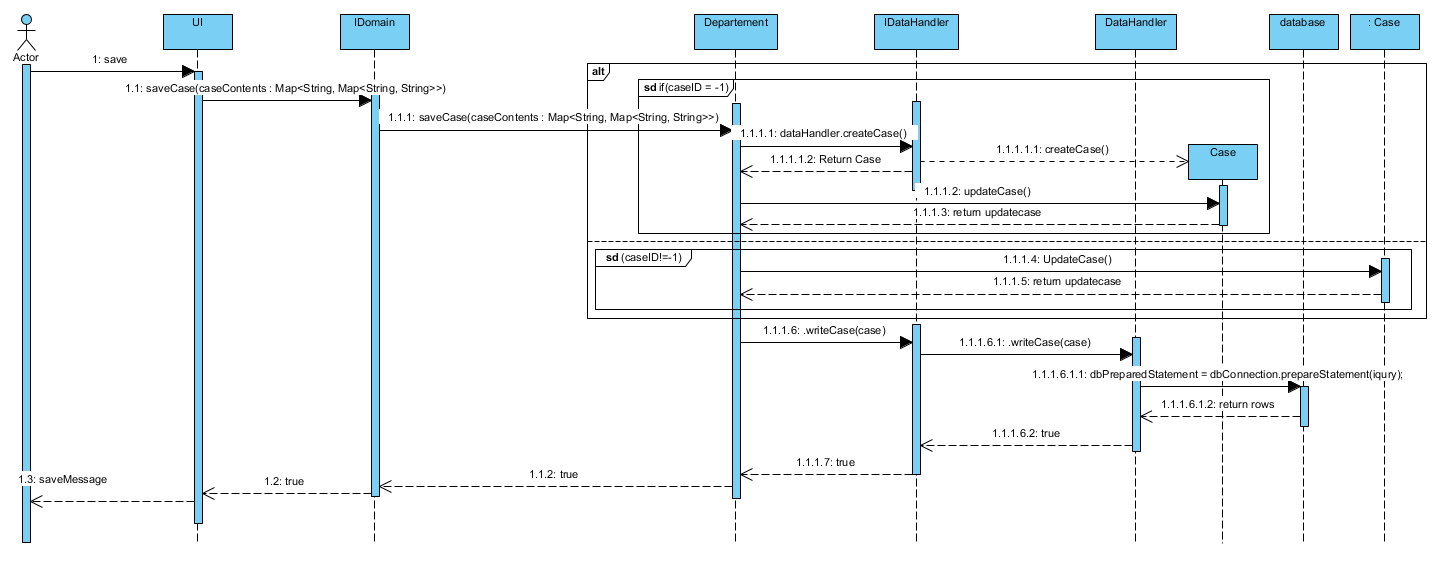
\includegraphics[width = \linewidth]{./PNG/design/odyn.PNG} 
  \caption{Sekvensdiagram for savecase}
  \label{fig:2savecase}
\end{figure}
\textbf{saveCase}
Når en aktør har udfyldt vilkårlige felter i sagsdokumenterne, kan denne data gemmes i databasen. \\
Når aktøren benytter ”1.save”, gemmes alt data der er indtastet i et contentsMap af typen ”Map\textless String, Map\textless String, String\textgreater \textgreater ”. Der benyttes et Map af Maps for at minimere koblingen. \\
Når contentsMap gemmes, benyttes metoden ”saveCase(…)” der sender den data igennem interfacet ”IDomain” ned til ”Department” facaden. Denne bliver pakket ud via metoden saveCase(…), i klassen Department, og tjekker på ”caseID” om det er lig med -1. Hvis dette er tilfældet, sender den Map ned videre igennem IDataHandler interfacet og ned til DataHandler. SaveCase(…) metoden i Datahandleren tjekker om der er en ny Case på caseID, hvis denne er -1, benyttes createCase() metoden der opretter et ”Case” objekt.\\
Hvis en Case allerede findes i Databasen, bliver updateCase() metoden kaldt, som opdatere ”Case” objektet og returner det opdaterede Case objekt. \\
Metoden som skriver i tilfældet af et eksisterende Case objekt eller et nyt Case objekt (1.1.1.6), benytter writeCase(…) metoden(1.1.1.6.1), som modtager et Case objekt og herefter skriver det ind i databasen ved at benytte en Prepared Statement. 
Hvis alle trin udføres succesfuldt, kvitteres der ”true” tilbage til aktøren. 
\begin{figure}[htb!]
  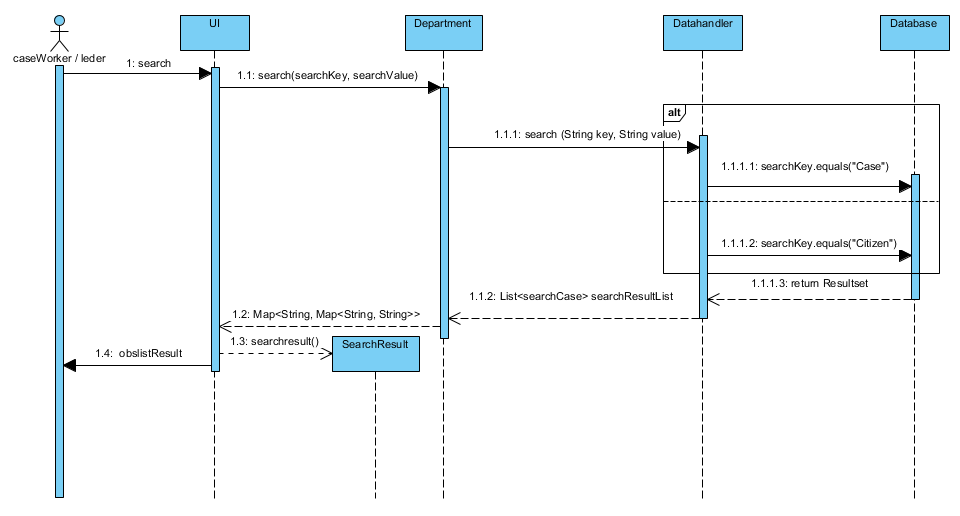
\includegraphics[scale = 0.55]{./PNG/design/seksearch.PNG} 
  \caption{Sekvensdiagram for search. Se interne bilag figur \ref{fig:seksearch}}
  \label{fig:2savecase}
\end{figure}
\\\textbf{Search}\\
1.	Personalet benytter søgefunktionen i systemet.\\
Denne bruges for at finde en eller flere sager på en given borger. \\
1.1.	En searchKey er blevet valgt i præsentationslaget og et searchValue er blevet\\ indtastet. Disse informationer sendes via Department metoden ”search(…)” , til domænelaget. \\
Den valgte ”searchKey” bruges til at vælge om der søges efter en specifik sag, eller sager der er relateret til en person. ”searchValue” bruges til at identificere de relevante informationer.\\
1.1.1.	Den valgte ”searchKey” bliver sendt videre som en ”String key” og searchValue bliver sendt videre som ”String value” i datahandler metoden search(…). \\
”StringKey” bestemmer hvilke SQL statement der skal bruges i persistenselaget. ”String value” er de værdier der skal matches i databasen. \\
1.1.1.1.	Her bliver der undersøgt om den ”String key” der er blevet modtaget, har værdien ”Case”\\
1.1.1.2.	 Her bliver der undersøgt om den ”String key” der er blevet modtaget, har værdien ”Citizen”. \\
Afhængigt af værdien, ”Case” eller ”Citizen”, vil en SQL kode blive kørt og hente informationer relateret til ”String value” fra 1.1.1.\\
1.1.1.3.	Databasen returner et ”ResultSet” med de værdier den har fundet. \\
Der bliver kun returneret data fra databasen, hvis ”departmentid” er i overensstemmelse med det der står i databasen. \\
1.1.2.	Data bliver pakket ind i  ”SearchCase” objekter og bliver gemt i en ”List\textless SearchCase\textgreater searchResultList” liste.\\
Denne liste sendes til domænelaget for at datapakken kan bearbejdes derfra. \\
1.2.	De modtagede ”SearchCase” objekter bliver læst og skrevet ind i ”searchResultMap”. Disse Maps bliver skrevet ind i HashMap ”searchResultList”.\\
Der bliver sendt et Map af Maps fordi ”SearchCase” objekterne ikke kan blive sendt videre til præsentationslaget. Vi minimerer kobling mellem lagende ved at skifte en liste af ”SearchCase” objekter  og udskifter dem med Map af Maps.\\
1.3.	Det modtagede ”Map\textless String, Map\textless String, String\textgreater \textgreater ” pakkes ud og opretter ”SearchResult” objekter af de inderste Maps. \\
1.4.	Alle ”SearchResult” objekter bliver tilføjet til en ”ObservableList\textless SearchResult\textgreater ”. \\
Der oprettes ”SearchResult” objekter for at kunne præsentere de modtagede informationer. Disse informationer tilføjes derefter til en ”ObservableList\textless SearchResult\textgreater ” liste for at ”TableView” kan præsentere de fundne informationer til brugeren. \\

\subsection{Implementering}

\subsection{Test}
